\documentclass{beamer}
\usetheme{Madrid}

\usepackage{cmap}
\usepackage[T2A]{fontenc}
\usepackage[russian,english]{babel}
\usepackage[utf8]{inputenc}
\usepackage{amsmath, amssymb}
\usepackage{minted}
\usepackage{hologo}

\usepackage{algorithm2e}
\usepackage{algorithmic}
\usepackage{float}

\usepackage{cancel}
\usepackage{ulem}

% \newtcbox{\mybox}{blank, on line, opacitytext=0.5}

\title[Ускорение обучения языковых моделей]{Методы оценки сложности текстовых данных для ускорения обучения языковых моделей с помощью обучения по плану}

\author[Сурков М.К.]{Сурков Максим Константинович\\
 	{\footnotesize Научный руководитель: Ямщиков Иван Павлович}
}
\institute[НИУ ВШЭ СПБ]{Санкт-Петербургская школа физико-математических и компьютерных наук \\ НИУ ВШЭ СПБ}
\date{9 июня 2021 г.}

\begin{document}

\frame{\titlepage}

\begin{frame}
	\frametitle{Мотивация. Применения}
	\begin{itemize}
		\item Основные задачи NLP и их приложения
			\begin{enumerate}
				\item классификация текстов (спам, грубая речь в соц. сетях)
				\item машинный перевод (яндекс.переводчик)
				\item построение вопросно-ответных систем (чат-боты)
			\end{enumerate}
		\item Как решаются задачи в NLP
			\begin{enumerate}
				\item Раньше: небольшие языковые модели
				\item Сейчас: трансформеры (большие нейронные сети со сложной архитектурой)
			\end{enumerate}
		\item В данной работе используется трансформер BERT
			\begin{enumerate}
				\item наиболее популярный
				\item имеет высокое качество
				\item имеет сравнительно небольшой размер $\Rightarrow$ удобно ставить эксперименты
			\end{enumerate}
	\end{itemize}
\end{frame}

\begin{frame}
	\frametitle{Мотивация. Обучение языковой модели}
	
	\begin{itemize}
		\item Для применения модели ее нужно обучить
		\item Обучение состоит из двух этапов:
			\begin{table}
				\begin{tabular}{|c|c|c|c|}
					\hline
					Этап & Время обучения & Корпус данных & Размер \\
					\hline
					Предобучение & 1-2 недели & Wikipedia & 3-600M \\
					&& BooksCorpus & 74M \\
					\hline
					Дообучение & 1-2 дня & HND & 600k-2M \\
					&& s140 & 1.6M\\
					&& ISWL & 200-230k \\
					&& QQP & 364k \\
					&& MNLI & 393k \\
					\hline
				\end{tabular}
			\end{table}
		\item Проблемы:
			\begin{itemize}
				\item {\bf долго} обучать
				\item нужно обрабатывать {\bf большие} объемы данных
			\end{itemize}
	\end{itemize}
\end{frame}

\begin{frame}
	\frametitle{Обучение по плану. Определение}
	
	Обучение по плану состоит из:
		\begin{enumerate}
			\item сортировки данных по {\bf метрике} сложности
			\item семплирования данных (алгоритм выборки данных из датасета)
		\end{enumerate}
	\vspace*{20pt}
	Пример\footnote{Platanios et al., Competence-based Curriculum Learning for Neural Machine Translation, 2019}
	\begin{columns}
		\column{0.5\textwidth}
		\begin{enumerate}
			\item сортируем тексты по длине (метрика=длина)
			\item семплируем данные из синей зоны
			\item синяя зона {\bf растет} вправо в течение обучения
			\item модель учится на все более сложных примерах
		\end{enumerate}
		\column{0.5\textwidth}
		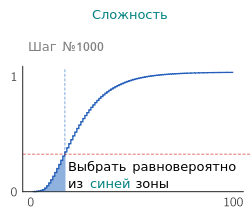
\includegraphics[scale=0.8]{acl19_algo.png}
	\end{columns}
\end{frame}

\begin{frame}
	\frametitle{Обзор существующих решений}

	\begin{enumerate}
		\item 
		В большинстве работ изучается влияние обучения по плану на задачах
		\begin{itemize}
			\item Машинного перевода (Platanios et al. (2019), Kocmi et al. (2017))
			\item NLU\footnote[1]{Построение вопросно-ответных систем} (Xu et al. (2020))
		\end{itemize}
	
		но не на
		\begin{itemize}
			\item {\bf Предобучении} языковых моделей
			\item {\bf Классификации} текстов
		\end{itemize}
	
		\item Обычно берутся очевидные метрики (например, длина)
		\begin{itemize}
			\item нет работ, которые расширяют множество метрик
		\end{itemize}		
	
		\item Подавляющее большинство статей использует обучение по плану для улучшения {\bf качества} модели, но {\bf не скорости} ее обучения
	\end{enumerate}
\end{frame}

\begin{frame}
	\frametitle{Цель и задачи}
	{\bf Цель:} исследовать возможность ускорения обучения языковой модели BERT на задачах предобучения модели и классификации текстов с помощью обучения по плану за счет применения улучшенной метрики сложности текстовых данных.
	
	{\bf Задачи:}
	\begin{enumerate}
		\item Предложить метрики оценки сложности текста
		\item Реализовать производительные алгоритмы вычисления предложенных метрик на больших корпусах данных
		\item Сравнить эффективность найденных метрик
		\item Исследовать влияние найденных метрик на скорость обучения языковой модели BERT на разных типах тренировочных данных
	\end{enumerate}
\end{frame}

\begin{frame}
	\frametitle{Поиск метрик}
	
	\begin{table}
		\begin{tabular}{|l|l|l|}
			\hline
			Метрика & Обозначение & Ссылка \\
			\hline
			Длина & длина & Platanios et al., 2019 \\
			\hline
			вероятность & правд. & Platanios et al., 2019 \\ 
			правдоподобия & & \\
			\hline
			ранг самого редкого & ранг & Xuan Zhang et al., 2018 \\
			слова в тексте & & \\
			\hline
			\hline
			$L_1$ норма вектора & TF-IDF & Эта работа \\
			TF-IDF & & \\
			\hline
			Excess Entropy & EE & адаптация \\
			& & Nihat Ay et al., 2006 \\
			\hline
			TSE & TSE & адаптация \\
			& & Nihat Ay et al., 2006 \\
			\hline
			модельная & MLM-loss & Эта работа \\
			\hline
			Среднее число токенов & TPW & Эта работа \\
			в слове & & \\
			\hline
		\end{tabular}
	\end{table}
	
\end{frame}

\begin{frame}
	\frametitle{Вычисление метрик}
	\begin{itemize}
		\item статистики
			\begin{enumerate}
				\item длина $\rightarrow$ число текстов с такой длиной
				\item $(i, x_i) \rightarrow$ число текстов, где $t_i = x_i$ 
				\item $(x_i)\rightarrow$ число текстов, где $x_i$ является последним токеном
				\item $(i, x_{i-1}, x_i) \rightarrow$ число текстов, где на $(i-1)$-й позиции стоит $x_{i-1}$, а на $i$-й позиции стоит $x_i$
				\item $x_i \rightarrow$ число текстов, в которых есть $x_i$
			\end{enumerate}
		\item сбор статистик в параллельном режиме (разделение по данным)
			\begin{table}
				\begin{tabular}{|c|c|}
					\hline
					Режим & Время \\
					\hline
					1 CPU & $\approx$ 2 недели \\
					5 CPU & $\approx$ 1-2 дня \\
					20 CPU & < 14 ч. \\
					40 CPU & < 6 ч. \\
					\hline
				\end{tabular}
			\end{table}
	\end{itemize}
\end{frame}

\begin{frame}
	\frametitle{Метод сравнения алгоритмов обучения}
	\begin{columns}
		\column{0.5\textwidth}
		
		\begin{itemize}
			\item Метрика -- объект изучения
			\item Хочется понять, как разные метрики влияют на скорость обучения
			\item Для этого нужно научиться сравнивать две метрики
			\item Для этого:
			\begin{enumerate}
				\item фиксируем все (кроме метрик)
				\item сравниваем среднее число шагов, необходимое для достижения порога
			\end{enumerate}
		\end{itemize}
		
		\column{0.5\textwidth}
		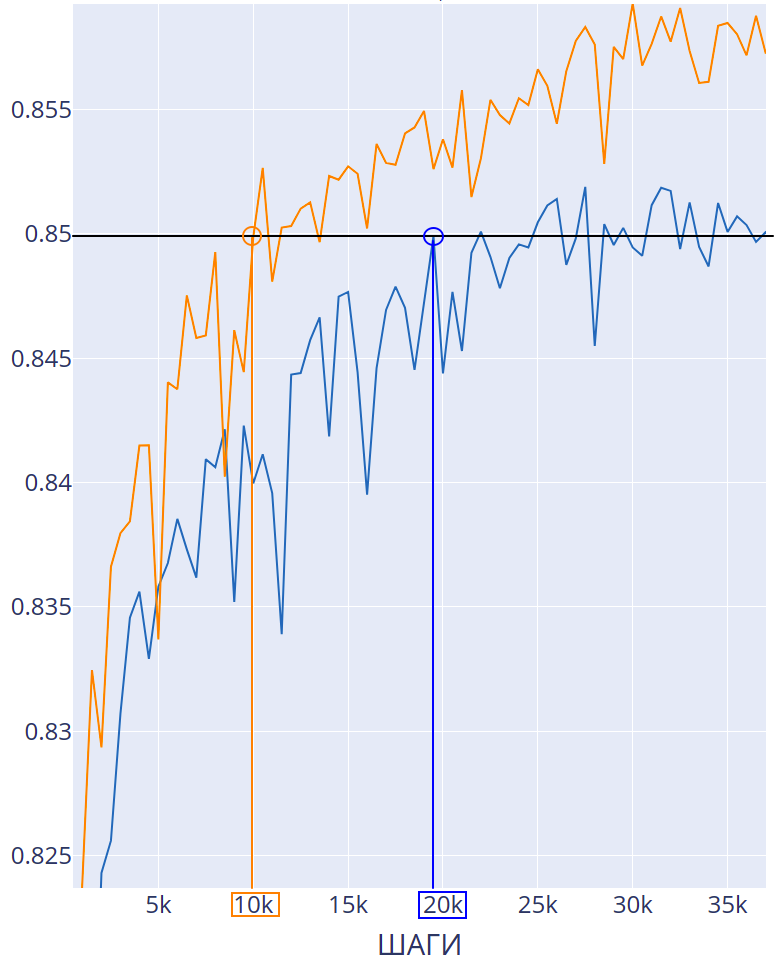
\includegraphics[scale=0.25]{compare}
	\end{columns}
\end{frame}

\begin{frame}
	\frametitle{Семплеры}
	В данной работе использованы следующие семплеры:

\noindent\makebox[\linewidth]{\rule{\paperwidth}{0.4pt}}
	\begin{columns}
		\column{0.5\textwidth}
		CB (Platanious et al., 2019) - префиксный семплер
		\column{0.5\textwidth}
		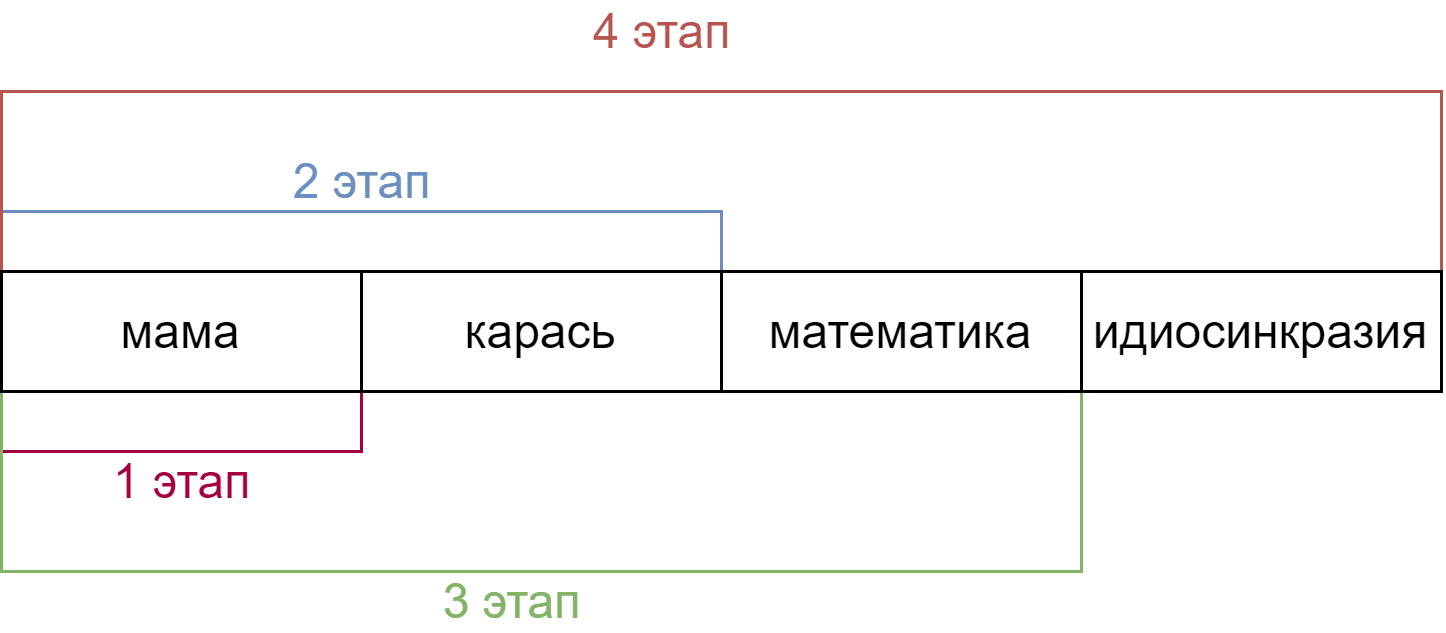
\includegraphics[scale=0.1]{prefix.png}
	\end{columns}
\noindent\makebox[\linewidth]{\rule{\paperwidth}{0.4pt}}
	\begin{columns}
		\column{0.5\textwidth}
		DB - суффиксный семплер
		\column{0.5\textwidth}
		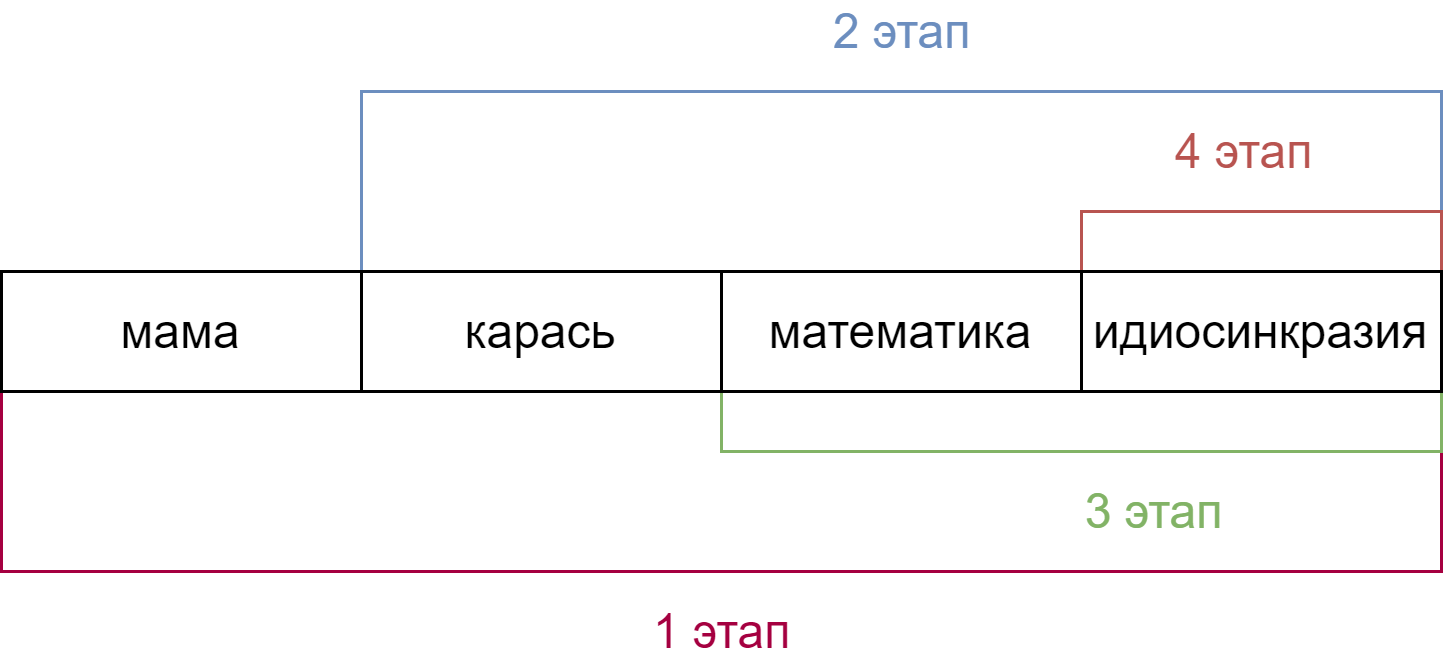
\includegraphics[scale=0.1]{suffix.png}
	\end{columns}
\noindent\makebox[\linewidth]{\rule{\paperwidth}{0.4pt}}
	\begin{columns}
		\column{0.5\textwidth}
		Hyp - оконный семплер
		\column{0.5\textwidth}
		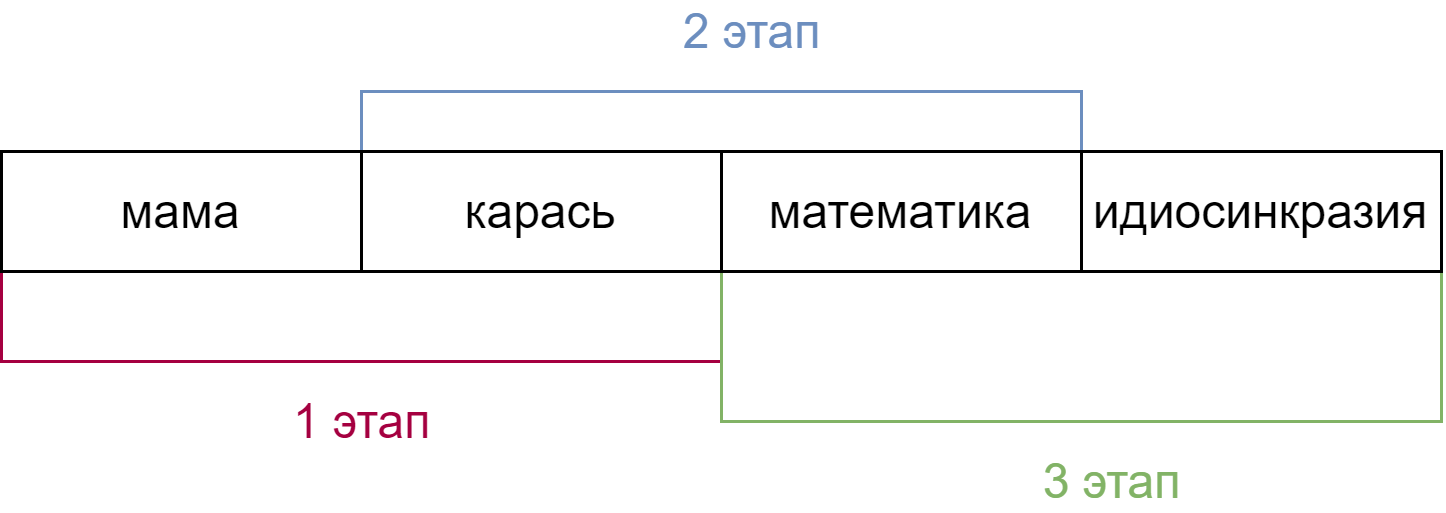
\includegraphics[scale=0.1]{window.png}
	\end{columns}
\noindent\makebox[\linewidth]{\rule{\paperwidth}{0.4pt}}
\end{frame}

\begin{frame}
	\frametitle{Семплеры}
	В данной работе использованы следующие семплеры:
	
	\begin{itemize}
		\item SS (shuffle-sort)
			\begin{enumerate}
				\item случайно поделим на батчи
				\item отсортируем батчи по средней сложности
			\end{enumerate}
		
		\item SM (sort-merge)
			\begin{enumerate}
				\item отсорируем по длине
				\item разобъем на группы
				\item каждую группу отсортируем по сложности
				\item строим батч из примеров каждоый группы
			\end{enumerate}
	\end{itemize}
\end{frame}

\begin{frame}
	\frametitle{Сравнение метрик: предобучение}
	\let\thefootnote\relax\footnotetext{стандартное отклонение $\delta \le 3k$ шагов}
	
	Датасет: BooksCorpus
	
	\begin{table}
		\begin{tabular}{|l|c|ccccc|c|}
			\hline
			Метрика & Порог & & & Семплеры & & & min loss \\
			\hline
			& & CB & DB & Hyp & SS & SM & \\
			\hline
			ранг & 2.00 & $\infty$ & 17.5k & {\bf 16.5k} & {\bf 16.5k} & 27k & {\bf 1.58} \\
			TF-IDF & 2.00 & $\infty$ & 34k & 35k & 37.5k & $\infty$ & 1.84 \\
			\hline
			\hline
			EE & 3.50 & $\infty$ & 4k & 3.5k & 4.5k & 9.5k & 2.25 \\
			TSE & 3.50 & $\infty$ & 9k & 9k & 8.5k & 18k & 2.60 \\
			правд. & 3.50 & $\infty$ & 13.5k & 13.5k & 15.5k & 50k & 2.83 \\
			длина & 3.50 & $\infty$ & 50.5k & $\infty$ & - & - & 3.45 \\
			\hline
			база & 2.00 & & & 9.5k & & & 1.58 \\
			\hline
		\end{tabular}
	\end{table}
	\begin{itemize}
		\item лучшая метрика -- максимальный ранг слова (замедляет в $2$ раза  {\bf без потери качества})
		\item обучение по плану замедляет обучение от 2 до 5 раз и ухудшает качество модели
	\end{itemize}
\end{frame}

\begin{frame}
	\frametitle{Сравнение метрик: классификация текстов}
	
	Датасеты: sentiment140 (результаты в таблице), HND
	\begin{table}
		\begin{tabular}{|l|c|ccccc|c|}
			\hline
			Метрика & Порог & & \multicolumn{3}{c}{Семплеры} & & Точность\\
			\hline
			& & CB & DB & Hyp & SS & SM & \\
			\hline
			{\bf ранг} & 85.5\% & 70k & 18.5k & 19.5k & {\bf 17k} & 19k & 86.7\% \\
			{\bf TF-IDF} & 85.5\% & 115.5k & 21.5k & 19.5k & {\bf 16.5k} & 22k & 86.7\% \\
			EE & 85.5\% & 59k & 19.3k & 23k & 20k & 19k & 86.7\% \\
			{\bf TSE} & 85.5\% & 95.5k & {\bf 16.5k} & 20.5k & 21.5k & 18k & 86.8\% \\
			правд. & 85.5\% & 112k & 17.5k & 21.5k & 17.5k & 21.5k & 86.7\% \\
			длина & 85.5\% & 112.5k & 20k & 19k & - & - & {\bf 86.2\%} \\
			MLM-loss & 85.5\% & 59.5k & 21k & 23.5k & 19.5k & 20k & {\bf 86.1\%} \\
			\hline
			база & 85.5\% & & & 17.5k & & & 87\% \\
			\hline
		\end{tabular}
	\end{table}
	\begin{itemize}
		\item лучшая конфигурация (TF-IDF+SS) ускоряет обучение до 3\% в среднем в сравнении с базой
		\item длина и MLM-loss уменьшают точность модели на 0.6\%
		\item в общем случае нет значительного ускорения обучения
	\end{itemize}
\end{frame}

\begin{frame}
	\frametitle{Влияние метрик на скорость обучения. Шум}
	\begin{itemize}
		\item Wu et al., When Do Curricula Work?, 2020 -- аналог для CV
		\item Для рассмотрения данного частного случая нужно искусственно добавить шум в данные
			\begin{enumerate}
				\item выберем $p \sim U[0, 0.4]$ -- уровень шума
				\item применим один из трех видов шумов к $p$ буквам в тексте
				\item виды шума:
					\begin{enumerate}
						\item {\bf клавиатурный} -- замена на случайного соседа по клавиатуре (Kumar et al. (2020)))
						\item ошибки произношения
						\item случайная перестановка двух символов в слове
					\end{enumerate}
			\end{enumerate}
		\item Оказалось, что метрика "уровень шума" ускоряет обучение до 2.15 раз на старте (семплер: DB, задача классификации текстов)
		
		\begin{columns}
			\column{0.5\textwidth}
				\begin{table}
					\begin{tabular}{lcc}
						\hline
						Метрики & Порог & Шаги \\
						\hline
						уровень шума & 83.5\% & 2k\\
						\hline
						база & 83.5\% & 4.3k\\
						\hline
					\end{tabular}
				\end{table}			
			\column{0.5\textwidth}
				\centering
				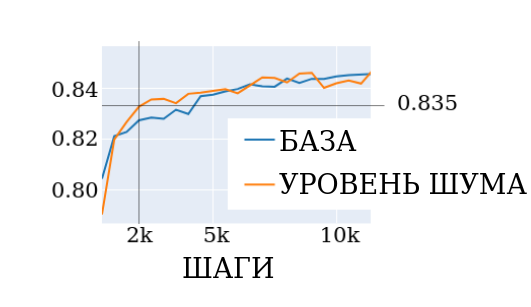
\includegraphics[scale=0.4]{keyboard_noise_level_short_prefix}
		\end{columns}
	\end{itemize}
\end{frame}

\begin{frame}
	\frametitle{Влияние метрик на скорость обучения. Шум}
	\begin{itemize}
		\item В реальности мы не обладаем информацией о количестве шума в конкретном примере $\Rightarrow$ нужно придумать метрику такую, что:
		\begin{enumerate}
			\item сильно коррелирует с уровнем шума
			\item не опирается на информацию о шуме
		\end{enumerate}
		\item Выяснилось, что подходит метрика TPW (среднее число токенов на слово)
			\begin{itemize}
				\item у шумных данных TPW больше $\Rightarrow$ модель сначала учится на чистых примерах, плавно переходя к более шумным
			\end{itemize}
		\item TPW ускоряет обучение в 1.72 раза для достижения 95\% (83.5\% из 87\%) итоговой точности (семплер: DB, задача классификации текстов)
			
		\vspace{-10pt}
			
		\begin{columns}
			\column{0.5\textwidth}
				\begin{table}
					\begin{tabular}{lcc}
						\hline
						Метрики & Порог & Шаги \\
						\hline
						TSE & 83.5\% & 5k\\
						TPW & 83.5\% & 2.5k\\
						\hline
						база & 83.5\% & 4.3k\\
						\hline
					\end{tabular}
				\end{table}			
			\column{0.5\textwidth}
				\centering
				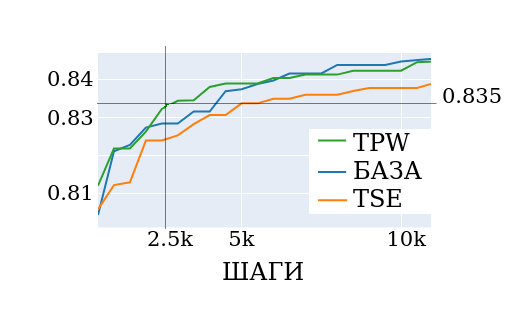
\includegraphics[scale=0.45]{keyboard_noise_TPW_win}		
		\end{columns}
	\end{itemize}
\end{frame}

\begin{frame}
	\frametitle{Результаты}
	\begin{enumerate}
		\item Предложен широкий спектр метрик оценки сложности текста
		\begin{itemize}
			\item метрики TSE и EE адаптированы под задачу обработки языка
		\end{itemize}
		\item Реализованы производительные алгоритмы подсчета метрик на больших объемах данных
		\item Результаты применения обучения по плану на задаче предобучения
			\begin{itemize}
				\item длина -- худшая метрика на предобучении (замедляет обучения до 12 раз, уменьшает качество модели)
				\item максимальный ранг слова -- лучшая метрика на предобучении (замедляет в $2$ раза {\bf без потери качества})
			\end{itemize}
		\item Дообучение на задаче классификации текстов
			\begin{itemize}
				\item лучшая конфигурация (TF-IDF+SS) ускоряет обучение до 3\% в среднем на классификации
				\item длина и MLM-loss уменьшают точность модели на 0.6\%
			\end{itemize}
		\item Шумные тренировочные данные
			\begin{itemize}
				\item 
				метрика TPW ускоряет обучение в {\bf 1.72 раза} для достижения 95\% итоговой точности на шумном корпусе данных
			\end{itemize}
	\end{enumerate}
\end{frame}

\appendix

\begin{frame}[label=supplemental,noframenumbering]
	\frametitle{Дополнительно: ссылки}
	\begin{itemize}
		\item Ay, N., Olbrich, E., Bertschinger, N., \& Jost, J. (2006, August). A\\\hspace{1cm}unifying framework for
		complexity measures of finite systems. In\\\hspace{1cm}Proceedings of ECCS (Vol. 6).
		\item Bengio, Y., Louradour, J., Collobert, R., \& Weston, J. (2009, June).\\\hspace{1cm}Curriculum learning. In
		Proceedings of the 26th annual \\\hspace{1cm}international conference on machine learning (pp.
		41-48).
		\item Brown, T. B., Mann, B., Ryder, N., Subbiah, M., Kaplan, J., \\\hspace{1cm}Dhariwal, P., ... \& Amodei, D.
		(2020). Language models are\\\hspace{1cm}few-shot learners. arXiv preprint arXiv:2005.14165.
		\item Devlin, J., Chang, M. W., Lee, K., \& Toutanova, K. (2018). Bert: \\\hspace{1cm}Pre-training of deep
		bidirectional transformers for language\\\hspace{1cm} understanding. arXiv preprint
		arXiv:1810.04805.
	\end{itemize}
\end{frame}

\begin{frame}[label=supplemental,noframenumbering]
	\frametitle{Дополнительно: ссылки}
	\begin{itemize}
		\item Hacohen, G., \& Weinshall, D. (2019, May). On the power of \\\hspace{1cm}curriculum learning in training
		deep networks. In International\\\hspace{1cm}Conference on Machine Learning (pp. 2535-2544).
		PMLR.
		\item Kocmi, T., \& Bojar, O. (2017). Curriculum learning and minibatch \\\hspace{1cm}bucketing in neural
		machine translation. arXiv preprint \\\hspace{1cm}arXiv:1707.09533.
		\item Kurdi, M. Z. (2020). Text Complexity Classification Based on \\\hspace{1cm}Linguistic Information:
		Application to Intelligent Tutoring of \\\hspace{1cm}ESL. arXiv preprint arXiv:2001.01863.
		\item Mermer, M. N., \& Amasyali, M. F. (2017). Scalable Curriculum \\\hspace{1cm}Learning for Artificial
		Neural Networks. IPSI BGD \\\hspace{1cm}TRANSACTIONS ON INTERNET RESEARCH, 13(2).
	\end{itemize}
\end{frame}

\begin{frame}[label=supplemental,noframenumbering]
	\frametitle{Дополнительно: ссылки}
	\begin{itemize}
		\item Narasimhan, S., Narasimhan, V. A. P. B. S., Karch, G., Rao, R., \\\hspace{1cm}Huang, J., Zhang, Y.,
		Ginsburg, B., Chitale, P., Sreenivas, S., \\\hspace{1cm}Mandava, S., Ginsburg, B., Forster, C., Mani,
		R., \& Kersten, K. \\\hspace{1cm}(2020, October 13). NVIDIA Clocks World’s Fastest BERT \\\hspace{1cm}Training
		Time and Largest Transformer Based Model, Paving \\\hspace{1cm}Path For Advanced
		Conversational AI. NVIDIA Developer Blog.
		\\\hspace{1cm}https://developer.nvidia.com/blog/training-bert-with-gpus/
		\item Platanios, E. A., Stretcu, O., Neubig, G., Poczos, B., \& Mitchell, T. \\\hspace{1cm}M. (2019).
		Competence-based curriculum learning for neural \\\hspace{1cm}machine translation. arXiv preprint
		arXiv:1903.09848.
		\item Sajjad, H., Dalvi, F., Durrani, N., \& Nakov, P. (2020). Poor Man's \\\hspace{1cm}BERT: Smaller and Faster
		Transformer Models. \\\hspace{1cm}arXiv preprint arXiv:2004.03844.
	\end{itemize}
\end{frame}


\begin{frame}[label=supplemental,noframenumbering]
	\frametitle{Дополнительно: ссылки}
	\begin{itemize}
		\item Shen, S., Dong, Z., Ye, J., Ma, L., Yao, Z., Gholami, A., Mahoney, M. \\\hspace{1cm}W., \& Keutzer, K.
		(2020). Q-BERT: Hessian Based Ultra Low \\\hspace{1cm}Precision Quantization of BERT.
		Proceedings of the AAAI \\\hspace{1cm}Conference on Artificial Intelligence, 34(05), 8815–8821.
		\\\hspace{1cm}https://doi.org/10.1609/aaai.v34i05.6409
		\item van der Sluis, F., \& van den Broek, E. L. (2010, August). Using \\\hspace{1cm}complexity measures in
		information retrieval. In Proceedings of \\\hspace{1cm}the third symposium on information
		interaction in context (pp. \\\hspace{1cm}383-388).
		\item Vaswani, A., Shazeer, N., Parmar, N., Uszkoreit, J., Jones, L., Gomez, \\\hspace{1cm}A. N., ... \&
		Polosukhin, I. (2017). Attention is all you need. \\\hspace{1cm}arXiv preprint arXiv:1706.03762.
	\end{itemize}
\end{frame}

\begin{frame}[label=supplemental,noframenumbering]
	\frametitle{Дополнительно: ссылки}
	\begin{itemize}
		\item Xu, B., Zhang, L., Mao, Z., Wang, Q., Xie, H., \& Zhang, Y. (2020). \\\hspace{1cm}Curriculum Learning for
		Natural Language Understanding. \\\hspace{1cm}Proceedings of the 58th Annual Meeting of the
		Association for \\\hspace{1cm}Computational Linguistics, 6095–6104.
		\\\hspace{1cm}https://doi.org/10.18653/v1/2020.acl-main.542
		\item Zhang, X., Kumar, G., Khayrallah, H., Murray, K., Gwinnup, J., \\\hspace{1cm}Martindale, M. J., ... \&
		Carpuat, M. (2018). An empirical \\\hspace{1cm}exploration of curriculum learning for neural
		machine \\\hspace{1cm}translation. arXiv preprint arXiv:1811.00739.
	\end{itemize}
\end{frame}

\begin{frame}[label=supplemental,noframenumbering]
	\frametitle{Дополнительно: Поиск метрик}
	\let\thefootnote\relax\footnotetext{Nihat Ay et al., A {\bf Unifying }Framework for Complexity Measures of Finite Systems, 2006}
	
	\begin{table}
		\begin{tabular}{c|c}
			\hline
			метрика & формула \\
			\hline
			Мультиинформация & $\sum\limits_{v\in V}H_p(X_v) - H_p(X_V)$ \\
			\hline
			{\bf Избыточная энтропия (EE)} & $\left[\sum\limits_{v\in V}H(X_{V\backslash\{v\}})\right] - (n - 1)H(X_V)$ \\
			\hline
			{\bf TSE} & $\sum\limits_{k=1}^{n-1}\frac{k}{n}C^{(k)}(X_V)$, где \\\\
			& $C^{(k)}(X_V) =$ \\\\
			& $\frac{n}{k\binom{n}{k}}\sum\limits_{A\subseteq V,|A|=k}H(X_A) - H(X_V)$ \\
			\hline
			Переходная информация & :( \\
			\hline
		\end{tabular}
	\end{table}
	
	\[
	V=\{1,\ldots,n\},
	X_V = (X_1,\ldots,X_n)
	\]
\end{frame}

\begin{frame}[label=supplemental,noframenumbering]
	\frametitle{Дополнительно: Адаптация EE и TSE под задачи обработки языка}
	
	\begin{enumerate}
		\item Образование совместной случайной величины
		\[
		T=(t_1, t_2, \ldots, t_{i-1},t_i,\ldots, t_n)
		\]
		\[
		t_i\rightarrow \xi^i_{t_i} =: \mu_i - \text{бинарная случайная величина}
		\]
		\[
		\downarrow
		\]
		\[
		\xi=(\xi^1_{t_1},\xi^2_{t_2},\ldots,\xi^{i-1}_{t_{i-1}},\xi^i_{t_i},\ldots,\xi^n_{t_n})
		\]
		\item Вычисление энтропии
		\[
		H(\mu) = \sum\limits_{i=1}^{n}H(\mu_i|\mu_1,\mu_2,\ldots,\mu_{i-1}) = \sum\limits_{i=1}^{n}H(\mu_i|\mu_{i-L},\ldots,\mu_{i-1})
		\]
		\item $L=1$
		\[
		H(\mu) = H(\mu_1) + H(\mu_2|\mu_1) + \ldots + H(\mu_i|\mu_{i-1}) + \ldots + H(\mu_n|\mu_{n-1})
		\]
	\end{enumerate}
\end{frame}

\begin{frame}[label=supplemental,noframenumbering]
	\frametitle{Дополнительно: Вычисление EE}
	\[
	EE(X) = \left[\sum\limits_{v\in V}H(X_{V\backslash\{v\}})\right] - (n - 1)H(X_V) = 
	\]
	\[
	\left[\sum\limits_{i=1}^{n}H(\mu_1,\ldots,\mu_{i-1},\mu_{i+1},\ldots,\mu_n)\right] - (n - 1)H(\mu)
	\]
	\begin{itemize}
		\item $\mathcal{O}(n^2)$
		\item $\mathcal{O}(n)$
		\[
		\sum\limits_{i=1}^{n}H(\mu_1,\ldots,\mu_{i-1},\mu_{i+1},\ldots,\mu_n) =\]
		\[ = \sum\limits_{i=1}^{n}H(\mu) - H(\mu_i|\mu_{i-1}) - H(\mu_{i+1}|\mu_i) + H(\mu_{i+1})\]
		\[
		EE(X) = \sum\limits_{i=2}^{n}H(\mu_i) - H(\mu_i|\mu_{i-1})= \sum\limits_{i=2}^{n}I(\mu_{i-1}\colon\mu_i)
		\]
	\end{itemize}
\end{frame}

\begin{frame}[label=supplemental,noframenumbering]
	\frametitle{Дополнительно: Вычисление TSE}
	\[
	\sum\limits_{k=1}^{n-1}\frac{k}{n}C^{(k)}(X_V)
	\]
	\[
	C^{(k)}(X_V) = \frac{n}{k\binom{n}{k}}\sum\limits_{A\subseteq V,|A|=k}H(X_A) - H(X_V) =
	\]
	\[
	= \frac{n}{k}\left[\frac{1}{\binom{n}{k}}\sum\limits_{A\subseteq V,|A|=k}H(X_A)\right] - H(X_V)
	\]
\end{frame}

\begin{frame}[label=supplemental,noframenumbering]
	\frametitle{Дополнительно: Вычисление TSE}
	\[
	\frac{1}{\binom{n}{k}}\sum\limits_{A\subseteq V,|A|=k}H(X_A) =
	\frac{1}{\binom{n}{k}}\sum\limits_{1 \le i_1 < i_2 < \ldots < i_k \le n}H(\mu_{i_1}, \mu_{i_2}, \ldots, \mu_{i_k})
	\]
	\begin{enumerate}
		\item $\mathcal{O^*}(2^n)$
		\item $\mathcal{O}(n^2)$ - динамическое программирование
		\item $\mathcal{O}(n)$
		\[
		\sum\limits_{i=1}^{n}A_iH(\mu_i) + \sum\limits_{i=2}^{n}B_iH(\mu_i|\mu_{i-1})
		\]
		\[
		A_i = 
		\begin{cases}
		\binom{n-2}{k-1}/\binom{n}{k}=\frac{k(n-k)}{n(n-1)},& i > 1 \\
		\binom{n-1}{k-1}/\binom{n}{k}=\frac k n,& i = 1
		\end{cases}
		\]
		\[
		B_i = \frac{\binom{n-2}{k-2}}{\binom{n}{k}} = \frac{k(k-1)}{n(n-1)}
		\]
	\end{enumerate}
\end{frame}

\begin{frame}[label=supplemental,noframenumbering]
	\frametitle{Результаты. Классификация. HND}
	\let\thefootnote\relax\footnotetext{стандартное отклонение $\delta \le 3k$ шагов}
	
	Датасет: Hyperpartisan News Detection
	
	\begin{table}
		\begin{tabular}{|l|c|ccccc|c|}
			\hline
			Метрика & Порог & & \multicolumn{3}{c}{Семплеры} & & Точность \\
			\hline
			 & & CB & DB & Hyp & SS & SM &\\
			\hline
			ранг & 92.9\%  & $\infty$ & 22k & {\bf 20.5k} & 22.5k & 39k & 93.6\% \\
			TF-IDF & 92.9\%  & $\infty$ & {\bf 19.5k} & 24k & 23.5k & 33k & 93.5\% \\
			EE & 92.9\%  & 71.5k & 25.5k & 22.5k & {\bf 19.5k} & 32.5k & 93.8\% \\
			TSE & 92.9\% & 56.5k & {\bf 21k} & 23k & 22k & 31k & 93.8\% \\
			правд. & 92.9\%  & $\infty$ & {\bf 20k} & 24k & {\bf 20k} & 30k & 93.8\% \\
			длина & 92.9\% & 55k & 23k & 22.5k & - & - & 93.7\% \\
			MLM-loss & 92.9\% & 23.5k & {\bf 18k} & 23k & 24k & 20k & {\bf 93.9\%} \\
			\hline
			база & 92.9\%  & & \multicolumn{3}{c}{22k} & & 93.8\% \\
			\hline
		\end{tabular}
	\end{table}
\end{frame}

\end{document}